\section{Authentiserungsmethoden}
Die Konfigurationsmöglichkeiten der strongSwan Open Source VPN Software sind enorm. Damit das Erfassen der Verbindungsdaten nicht all zu unübersichtlich wird, beschränken wir uns auf die häufigst verwendeten Szenarien.

\begin{enumerate}
	\item X.509 Zertifikat und privater RSA/ECDSA Schlüssel
	\item EAP mit Benutzername/Passwort
	\item Zweirunden-Authentisierung mit Methode 1) gefolgt von Methode 2)
	\item EAP-TLS mit X.509 Zertifikat und privatem RSA/ECDSA Schlüssel
\end{enumerate}

Nachfolgend wird auf die jeweiligen Authentiserungsmethoden im Detail eingegangen. Bei der Verwendeten Notation der Konfiguration handelt es sich um Python ordered Dictionaries.\\
Die Clientseite wurde mit Hilfe der strongMan Applikation erstellt. Die Serverseite dient als Pendant dazu und ist als ein funktionstüchtiges Beispiel aufgeführt.

\subsubsection{Konfiguration}
Die Tabelle Konfiguration beschreibt einige Key Parameter, welche durch die strongMan Applikation gesetzt werden. Eine komplette Übersicht über die Paramter findet sich im strongSwan Repository auf Github\footnote{\url{https://github.com/strongswan/strongswan/tree/master/src/libcharon/plugins/vici}}, weiter kann die Dokumentation von swanctl\footnote{\url{https://wiki.strongswan.org/projects/strongswan/wiki/Swanctlconf}} als Hilfestellung hinzugezogen werden.\\
\begin{table}[H]
\centering
    \begin{tabular}{|p{0.2\textwidth}|p{0.2\textwidth}|p{0.5\textwidth}|}
    \hline
    \rowcolor{lightblue}
    Parameter & Wert & Erklärung \\ \hline
	vips	&	0.0.0.0,  :: & Virtuelle IP, welche dem Client vom Server zugewiesen wird. 0.0.0.0 und :: dienen als Wildcard-Adressen für IPv4 und IPv6, damit wird jede virtuelle IP akzeptiert.	\\ \hline
	version & 2 & IKE Version, es wird nur die Version 2 von strongMan verwendet \\ \hline
	auth & pubkey, eap, eap-tls & Definiert die verwendete Authentisierungsmethode. \\ \hline
	round & 1, 2 & Wird von Certificate + EAP benötigt, da es zwei Authentiserungsrunden hat. Der Parameter wird erst ab strongSwan Version 5.4.0 unterstützt. \\ \hline
	certs & Bytes & Byte Repräsentation des Benutzer-Zertifikates	\\ \hline
	cacerts & Bytes & Byte Repräsentation des Server-Zertifikates	\\ \hline
	\end{tabular}
    \caption[Konfiguration]{Konfiguration}
\end{table}
\newpage

\subsubsection{IKEv2 Certificate}
Die Authentisierung zwischen Client und Server findet auf Basis eines X.509 Zertifikats und privater RSA/ECDSA Schlüssel statt.\\
\noindent\begin{minipage}[t]{0.5\textwidth}
\vspace{0pt}
\paragraph{Eingabefelder}\mbox{}\medskip
    \begin{figure}[H]
    	\centering
    	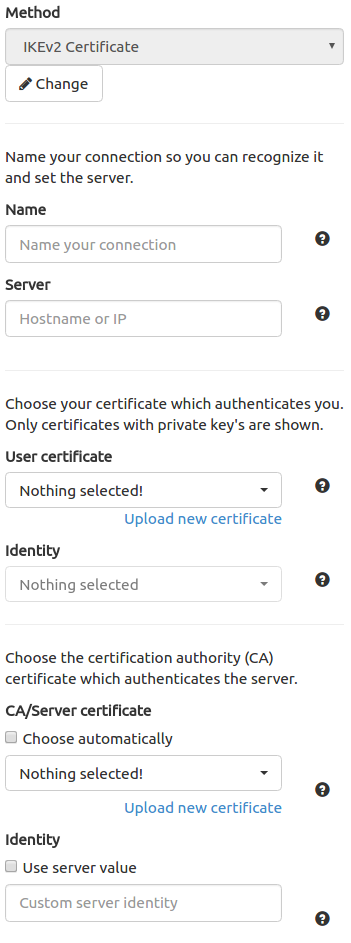
\includegraphics[width=200pt]{images/ike_cert.png}
    	\caption{IKEv2 Certificate}
    \end{figure}
\end{minipage}
\hfill
\begin{minipage}[t]{0.5\textwidth}
\vspace{0pt}
\paragraph{Beschreibung}\mbox{}\\
\paragraph{Name}\mbox{}\\
\hspace*{18pt}Ordered Dictionary: 'Bezeichner'\\
Eindeutige Bezeichnung für die Verbindung \\

\paragraph{Server}\mbox{}\\
\hspace*{18pt}Ordered Dictionary: remote\_addrs\\
Hostname oder IP des Servers\\

\paragraph{User certificate}\mbox{}\\
\hspace*{18pt}Ordered Dictionary: local.certs\\
Auswahl der Benutzerzertifikate. Im ordered Dictionary wird der komplette DER-Container in Binärer Form übermittelt.\\

\paragraph{Identitiy}\mbox{}\\
\hspace*{18pt}Ordered Dictionary: local.certs\\
Auswahl der Benutzerzertifikate. Im ordered Dictionary wird der komplette DER-Container in Binärer Form übermittelt.\\

\paragraph{User certificate}\mbox{}\\
\hspace*{18pt}Ordered Dictionary: local.id\\
Auswahl zwischen Subject Alternative Name und Distinguished Name. Standardmässig wird der Distinguished Name gesetzt, somit wird nur bei Auswahl eines Subject Alternative Name die local.id in das ordered Dictionary geschrieben.\\

\paragraph{CA/Server certificate}\mbox{}\\
\hspace*{18pt}Ordered Dictionary: remote.cacerts\\
Die automatische Auswahl bewirkt, dass alle CA/Server Zertifikate an den strongSwan übergeben werden und dieser selbständig entscheidet. Ansonsten wird das passende manuell ausgewählt.\\

\paragraph{Identity}\mbox{}\\
\hspace*{18pt}Ordered Dictionary: remote.id\\
Bezeichner für die Server identifikation. Per Default wird der \textbf{Server} Eintrag übernommen. Ansonsten auch manuell setzbar.\\

\end{minipage}
\newpage

\noindent\begin{minipage}[t]{0.5\textwidth}
\vspace{0pt}
\paragraph{Client}\mbox{}\medskip
\begin{lstlisting}[style=BashInputStyle]
{
    "cert": {
        "remote_addrs": [
            "gateway"
        ],
        "vips": [
            "0.0.0.0",
            "::"
        ],
        "version": 2,
        "proposals": [
            "aes128-sha256-modp2048"
        ],
        "children": {
            "cert": {
                "remote_ts": [
                    "::/0",
                    "0.0.0.0/0"
                ],
                "esp_proposals": [
                    ''aes128gcm128-
                    modp2048''
                ]
            }
        },
        "local": {
            "round": 1,
            "auth": "pubkey"
            "certs": [
                "b'bytes_of_cert'"
            ]
        },
        "remote-cert": {
            "round": 1,
            "auth": "pubkey",
            "id": "moon.strongswan.org"
            "cacerts": [
                "b'bytes_of_cert'"
            ]
        }
    }
}
\end{lstlisting}
\end{minipage}
\hfill
\begin{minipage}[t]{0.5\textwidth}
\vspace{0pt}
\paragraph{Server}\mbox{}\medskip
\begin{lstlisting}[style=BashInputStyle]
{
    "server-cert": {
        "pools": [
            "server-pool"
        ],
        "local": {
            "auth": "pubkey",
            "id": "moon.strongswan.org",
            "certs": [
                "moonCert.pem"
            ]
        },
        "remote": {
            "auth": "pubkey"
        },
        "version": 2,
        "proposals": [
            "aes128-sha256-modp2048"
        ],
        "children": {
            "server-cert": {
                "esp_proposals": [
                    ''aes128gcm128-
                    modp2048''
                ]
            }
        }
   }
}
\end{lstlisting}
\hspace*{18pt}\textbf{Pools}\mbox{}\medskip
\begin{lstlisting}[style=BashInputStyle]
"server-pool": {
    "addrs": "10.6.0.0/24"
}
\end{lstlisting}
\end{minipage}
\newpage



\subsubsection{IKEv2 EAP (Username/Password)}
Die Authentisierung zwischen Client und Server findet auf Basis von EAP mit Hilfe eines Benutzernamens und Passwortes statt.
Die \textbf{eap-id} ist eine Referenz auf das Secret.

\noindent\begin{minipage}[t]{0.5\textwidth}
\vspace{0pt}
\paragraph{Eingabefelder}\mbox{}\medskip
    \begin{figure}[H]
    	\centering
    	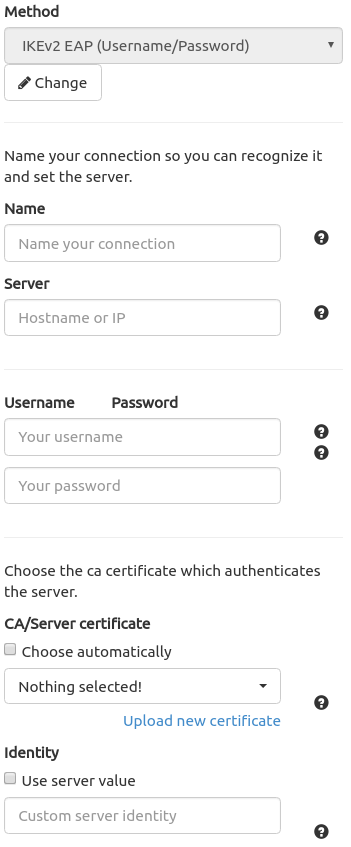
\includegraphics[width=200pt]{images/ike_eap.png}
    	\caption{IKEv2 EAP}
    \end{figure}
\end{minipage}
\hfill
\begin{minipage}[t]{0.5\textwidth}
\vspace{0pt}
\paragraph{Beschreibung}\mbox{}\\
\paragraph{Username}\mbox{}\\
\hspace*{18pt}Ordered Dictionary: secrets.id, local.eap\_id\\
Username wird als als Referenz zwischen den Secrets und der local Section verwendet. \\

\paragraph{Password}\mbox{}\\
\hspace*{18pt}Ordered Dictionary: secrets.data\\
Passwort für die EAP Authentisierung wird verschlüsselt in der Datenbank gespeichert.\\

\end{minipage}
\newpage


\noindent\begin{minipage}[t]{0.5\textwidth}
\vspace{0pt}
\paragraph{Client}\mbox{}\medskip
\begin{lstlisting}[style=BashInputStyle]
{
    "eap": {
        "remote_addrs": [
            "gateway"
        ],
        "vips": [
            "0.0.0.0",
            "::"
        ],
        "version": 2,
        "proposals": [
            "aes128-sha256-modp2048"
        ],
        "children": {
            "eap": {
                "remote_ts": [
                    "::/0",
                    "0.0.0.0/0"
                ],
                "esp_proposals": [
                    ''aes128gcm128-
                    modp2048''
                ]
            }
        },
        "local-eap": {
            "round": 1,
            "auth": "eap",
            "eap_id": "eap-test"
        },
        "remote-cert": {
            "round": 1,
            "auth": "pubkey",
            "id": "moon.strongswan.org"
        }
    }
}
\end{lstlisting}
\hspace*{18pt}\textbf{Secrets}\mbox{}\medskip
\begin{lstlisting}[style=BashInputStyle]
{
    "data": "test",
    "id": "eap-test",
    "type": "EAP"
}
\end{lstlisting}
\end{minipage}
\hfill
\begin{minipage}[t]{0.5\textwidth}
\vspace{0pt}
\paragraph{Server}\mbox{}\medskip
\begin{lstlisting}[style=BashInputStyle]
{
    "server-eap": {
        "pools": [
            "server-pool"
        ],
        "local": {
            "auth": "pubkey",
            "id": "moon.strongswan.org",
            "certs": [
                "moonCert.pem"
            ]
        },
        "remote-eap": {
            "auth": "eap-md5"
        },
        "version": 2,
        "proposals": [
            "aes128-sha256-modp2048"
        ],
        "children": {
            "server-eap": {
                "esp_proposals": [
                    ''aes128gcm128-
                    modp2048''
                ]
            }
        }
   }
}
\end{lstlisting}
\hspace*{18pt}\textbf{Secrets}\mbox{}\medskip
\begin{lstlisting}[style=BashInputStyle]
{
    "data": "test",
    "id": "eap-test",
    "type": "EAP"
}
\end{lstlisting}
\hspace*{18pt}\textbf{Pools}\mbox{}\medskip
\begin{lstlisting}[style=BashInputStyle]
"server-pool": {
    "addrs": "10.6.0.0/24"
}
\end{lstlisting}
\end{minipage}


\subsubsection{IKEv2 EAP-TLS}
Mit der EAP-TLS Konfiguration wird ohne separate IKEv2 Authentifikation ein Verbindung aufgebaut, die das TLS Client- und Serverzertifikat verwendet.\\
\noindent\begin{minipage}[t]{0.5\textwidth}
\vspace{0pt}
\paragraph{Client}\mbox{}\medskip
\begin{lstlisting}[style=BashInputStyle]
{
    "eap-tls": {
        "remote_addrs": [
            "gateway"
        ],
        "vips": [
            "0.0.0.0",
            "::"
        ],
        "version": 2,
        "proposals": [
            "aes128-sha256-modp2048"
        ],
        "children": {
            "eap-tls": {
                "remote_ts": [
                    "::/0",
                    "0.0.0.0/0"
                ],
                "esp_proposals": [
                    ''aes128gcm128
                    -modp2048''
                ]
            }
        },
        "local-eap-tls": {
            "round": 1,
            "auth": "eap-tls",
            "eap_id": "eap-test"
        },
        "remote-cert": {
            "round": 1,
            "auth": "pubkey",
            "id": "moon.strongswan.org"
        }
    }
}
\end{lstlisting}
\hspace*{18pt}\textbf{Secrets}\mbox{}\medskip
\begin{lstlisting}[style=BashInputStyle]
{
    "data": "test",
    "id": "eap-test",
    "type": "EAP"
}
\end{lstlisting}
\end{minipage}
\hfill
\begin{minipage}[t]{0.5\textwidth}
\vspace{0pt}
\paragraph{Server}\mbox{}\medskip
\begin{lstlisting}[style=BashInputStyle]
{
    "server-eap-tls": {
        "pools": [
            "server-pool"
        ],
        "local": {
            "auth": "pubkey",
            "id": "moon.strongswan.org",
            "certs": [
                "moonCert.pem"
            ]
        },
        "remote-eap": {
            "auth": "eap-dynamic"
            "eap_id": "eap-test"
        },
        "version": 2,
        "proposals": [
            "aes128-sha256-modp2048"
        ],
        "children": {
            "server-eap-tls": {
                "esp_proposals": [
                    ''aes128gcm128-
                    modp2048''
                ]
            }
        }
   }
}
\end{lstlisting}
\hspace*{18pt}\textbf{Secrets}\mbox{}\medskip
\begin{lstlisting}[style=BashInputStyle]
{
    "data": "test",
    "id": "eap-test",
    "type": "EAP"
}
\end{lstlisting}
\hspace*{18pt}\textbf{Pools}\mbox{}\medskip
\begin{lstlisting}[style=BashInputStyle]
"server-pool": {
    "addrs": "10.6.0.0/24"
}
\end{lstlisting}
\end{minipage}
\newpage


\subsubsection{	IKEv2 Certificate + EAP (Username/Password)}
Zwei Runden Authentisierung, basierend auf der Kombination von EAP und Zertifikat.\\
\noindent\begin{minipage}[t]{0.5\textwidth}
\vspace{0pt}
\paragraph{Client}\mbox{}\medskip
\begin{lstlisting}[style=BashInputStyle]
{
    "eap-cert": {
        "remote_addrs": [
            "gateway"
        ],
        "vips": [
            "0.0.0.0",
            "::"
        ],
        "version": 2,
        "proposals": [
            "aes128-sha256-modp2048"
        ],
        "children": {
            "eap-cert": {
                "remote_ts": [
                    "::/0",
                    "0.0.0.0/0"
                ],
                "esp_proposals": [
                    ''aes128gcm128-
                    modp2048''
                ]
            }
        },
        "local-cert": {
            "round": 1,
            "auth": "pubkey"
        },
        "local-eap": {
            "round": 2,
            "auth": "eap",
            "eap_id": "eap-test"
        },
        "remote-eap-cert": {
            "round": 1,
            "auth": "pubkey",
            "id": "moon.strongswan.org"
        }
    }
}
\end{lstlisting}
\hspace*{18pt}\textbf{Secrets}\mbox{}\medskip
\begin{lstlisting}[style=BashInputStyle]
{   "data": "test",
    "id": "eap-test",
    "type": "EAP"   }
\end{lstlisting}
\end{minipage}
\hfill
\begin{minipage}[t]{0.5\textwidth}
\vspace{0pt}
\paragraph{Server}\mbox{}\medskip
\begin{lstlisting}[style=BashInputStyle]
{
    "server-cert-eap": {
        "pools": [
            "server-pool"
        ],
        "local": {
            "auth": "pubkey",
            "id": "moon.strongswan.org",
            "certs": [
                "moonCert.pem"
            ]
        },
        "remote": {
            "auth": "pubkey",
            "round": 1
        },
        "remote-eap": {
            "auth": "eap-md5",
            "eap_id": "eap-test",
            "round": 2
        },
        "version": 2,
        "proposals": [
            "aes128-sha256-modp2048"
        ],
        "children": {
            "server-cert-eap": {
                "esp_proposals": [
                    ''aes128gcm128-
                    modp2048''
                ]
            }
        }
   }
}
\end{lstlisting}
\hspace*{18pt}\textbf{Secrets}\mbox{}\medskip
\begin{lstlisting}[style=BashInputStyle]
{   
    "data": "test",
    "id": "eap-test",
    "type": "EAP"   
}
\end{lstlisting}
\hspace*{18pt}\textbf{Pools}\mbox{}\medskip
\begin{lstlisting}[style=BashInputStyle]
"server-pool": {
    "addrs": "10.6.0.0/24"
}
\end{lstlisting}
\end{minipage}
\nolinebreak
\nopagebreak